\documentclass[]{final_report}
\usepackage{graphicx}
\usepackage{hyperref}
\usepackage{titlesec}
\usepackage[utf8]{inputenc}
\usepackage[backend=biber, style=ieee]{biblatex}
\usepackage{amsmath}
\usepackage{amssymb}
\usepackage{float}
\usepackage{tabularx} % Needed for the X column type
\usepackage{booktabs} % For prettier tables
\usepackage{lipsum}   % For dummy text


\addbibresource{fyp.bib}
\usepackage{amsthm}
\theoremstyle{definition}
\newtheorem{definition}{Definition}[chapter]
\newtheorem{basic}{Basic Definition}

%%%%%%%%%%%%%%%%%%%%%%
%%% Input project details
\def\studentname{Jude Asare}
\def\reportyear{2023/2024}
\def\projecttitle{Implementing the PKCS\#1 v1.5 Signature Scheme with provably secure parameters}
\def\supervisorname{Saqib Kakvi}
\def\degree{MSci (Hons) in Computer Science (Information Security)}
\def\fullOrHalfUnit{MSci} 
\def\finalOrInterim{Interim Report} 
\begin{document}

\maketitle


%%%%%%%%%%%%%%%%%%%%%%
%%% Declaration

\chapter*{Declaration}

This report has been prepared on the basis of my own work. Where other published and unpublished source materials have been used, these have been acknowledged.

\vskip3em

Word Count: 

\vskip3em

Student Name: \studentname

\vskip3em

Date of Submission: 

\vskip3em

Signature:

\newpage

%%%%%%%%%%%%%%%%%%%%%%
%%% Table of Contents
\tableofcontents\pdfbookmark[0]{Table of Contents}{toc}\newpage

%%%%%%%%%%%%%%%%%%%%%%
%%% Project Spec

\chapter*{Project Specification}
\addcontentsline{toc}{chapter}{Project Specification}
% Begin reduced spacing
{
\titlespacing*{\section}
{0pt}{1.4ex plus 1ex minus .2ex}{1.0ex plus .2ex}

\section*{Background:}
The PKCS\#1 v1.5 signature scheme is one of the most widely used signature schemes in practice, mainly due to its use in TLS. While it has been used for decades, there was no security proof for the scheme, which cast some doubt on its usability. Although RSA-PSS has been suggested as a replacement, it is randomised and is more computationally expensive, so keeping PKCS\#1 is preferable. in 2018 Jager, Kakvi and May presented a proof of security for the PKCS\#1 v1.5 signature schemes, but only if larger parameters are used. The question to be answered is how much of an overhead is introduced by using the provably secure parameters.

\section*{Prerequisites:}
Some undergraduate mathematical background e.g. linear algebra, number theory is useful. Experience implementing programs that work with large numbers is a bonus.

\section*{Early Deliverables}
\begin{enumerate}
    \item A report describing provable security and how it affects parameter choices.
    \item A report motivating the use of provably secure parameters.
    \item Proof of concept implementation of parametrisable RSA key generation.
\end{enumerate}

\section*{Final Deliverables}
\begin{enumerate}
    \item An implementation of PKCS\#1 v1.5 signatures scheme with provably secure and standard parameters.
    \item A benchmarking program to compare the scheme with provably secure parameters and standard ones.
    \item Report explaining the implementation of RSA based schemes.
    \item Report explaining relevant cryptographic concepts e.g. definitions of digital signatures, notions of security, etc.
\end{enumerate}

\section*{Reading}
\begin{itemize}
    \item \href{https://eprint.iacr.org/2018/855.pdf}{https://eprint.iacr.org/2018/855.pdf}
    \item \href{https://datatracker.ietf.org/doc/html/rfc8017}{https://datatracker.ietf.org/doc/html/rfc8017}
    \item \href{https://www.ecrypt.eu.org/csa/documents/D5.4-FinalAlgKeySizeProt.pdf}{https://www.ecrypt.eu.org/csa/documents/D5.4-FinalAlgKeySizeProt.pdf}
    \item \href{https://www.openssl.org/docs/manmaster/man1/openssl-speed.html}{https://www.openssl.org/docs/manmaster/man1/openssl-speed.html}
\end{itemize}
}
% End reduced spacing


%%%%%%%%%%%%%%%%%%%%%%
%%% Your Abstract here

\begin{abstract}



The PKCS\#1 v1.5 digital signature scheme has been widely utilised in protocols such as SSH, DNSSEC, IKE, and most prominently, in TLS up to version 1.2. Since its inception in 1998 \cite{rfc2313} it has played a pivotal role in the landscape of digital security comprising the most widely used digital signature scheme in practice. The scheme, renowned for its straightforwardness and expedited verification capabilities, has seen persistent integration across diverse cryptographic systems. 

Nevertheless, amidst its widespread acceptance, it's been marred by several challenges. Among these are the targeting of latent vulnerabilities \cite{bleichenbacher1998chosen, coppersmith1996low, coron2000new, 10.1007/978-3-540-45238-6_33, degabriele2012joint, bardou2012efficient, meyer2014revisiting, zhang2014cross, jager2015security, jager2015practical, bock2018return} inherent to its associated encryption paradigm \cite{rfc2313} which aided in revealing potential weaknesses in the signature scheme itself (\cite{finney2006bleichenbacher}, \cite{kuhn2008variants}, \cite{cve-2006-4790, cve-2006-4340, bugzilla-1064636, intel-berserk-vulnerability, josefsson-signature-forgery, valsorda-bleichenbacher-forgery}) and a glaring absence of a rigorous security proof that validates its resilience.

Even though alternatives like RSA-PSS offer provable security (\cite{bellare1996exact}, \cite{jonsson2001security}), they come with inherent problem, such as the introduction of randomness and a hike in computational complexity. These issues have created reservations for its wholesale adoption in place of PKCS\#1 v1.5 e.g., RSA-PSS and was only upgraded to a requirement for new applications in PKCS\#1 v2.2 \cite{rfc8017} long after initially being suggested as the replacement for PKCS\#1 v1.5 in PKCS\#1 v2.1 \cite{rfc3447}. Imperative requirements of backward compatibility and interoperability have been the main detractors of the aversion to replacing PKCS\#1 v1.5 and while RSA-PSS is now required in new applications, they entail retaining PKCS\#1 v1.5 in some form at the very least, as a preferable choice.
 
A significant breakthrough came in 2018 when Jager, Kakvi, and May \cite{jager2018security} provided a security proof for the PKCS\#1 v1.5 Signature scheme building on the work of Coron \cite{coron2002security}. Although still requiring the adoption of larger cryptographic parameters deviating slightly from standard use, their methods were flexible enough to show instantiations in practice such that the improved proofs apply. Benefits not limited to PKCS\#1 v1.5, their work also offered insights enabling the proof to apply to other deterministic RSA signature schemes, with similar construction patterns including ISO/IEC 9796-2 and ANSI X9.31 schemes.

Guided by this revelation, this project seeks to concretely implement these signature schemes, with a primary emphasis on the PKCS\#1 v1.5 signature scheme, using the aforementioned provably secure parameters. This project aims not only to showcase its practicality, but also as a primary objective dissect the computational burdens these parameters introduce into deterministic RSA schemes. This objective is supplemented by supporting objectives to produce algorithms that facilitate its implementation with both provably secure parameters and separately standard parameters. From there the aim is to produce an all-incorporative user-interfaced benchmarking program to explore aforementioned overhead across standards. 
\newpage
\end{abstract}
\newpage


%%%%%%%%%%%%%%%%%%%%%%
%%% Introduction
\chapter{Introduction}


\section{Importance}

The PKCS\#1 v1.5 digital signature scheme, rooted in RSA's hash-and-sign framework, has emerged as the de facto standard for digital signatures since its 1998 introduction \cite{rfc2313}, despite lacking formal security proofs. Essential in security-focused network protocols like SSH, DNSSEC, IKE, and pre-TLS 1.3 X.509 certificates \cite{schaad2005additional}, its simplicity fosters broad adoption from its outset, straightforward implementation across programming languages, and speedy verifications relative to alternatives like DSA or ECDS  \cite{jager2018security}. Many legacy systems and protocols continue to rely on RSA PKCS\#1 v1.5 signatures for the sake of backward compatibility alone. The deep integration of this scheme into various applications, sometimes even at the hardware level, suggests that PKCS\#1 v1.5 is likely to remain in use for the foreseeable future.

\section{Security Concerns and the Drive for Provable Security}
This extensive usage has not been without its share of security concerns. Several studies \cite{bleichenbacher1998chosen, coppersmith1996low, coron2000new, 10.1007/978-3-540-45238-6_33, degabriele2012joint, bardou2012efficient, meyer2014revisiting, zhang2014cross, jager2015security, jager2015practical, bock2018return} have highlighted vulnerabilities in the accompanying PKCS\#1 v1.5 encryption scheme, primarily due to the Bleichenbacher padding oracle attacks \cite{bleichenbacher1998chosen}. Although these attacks did not directly compromise the PKCS\#1 v1.5 signature scheme, they did reveal potential weaknesses (\cite{finney2006bleichenbacher}, \cite{kuhn2008variants}, \cite{cve-2006-4790, cve-2006-4340, bugzilla-1064636, intel-berserk-vulnerability, josefsson-signature-forgery, valsorda-bleichenbacher-forgery}) related to certain checks omitted in signature verification implementations. Notable failures have indeed occurred in major implementations, as witnessed in the case of Python-RSA in 2016  \cite{valsorda-bleichenbacher-forgery}. Furthermore, until 2018 no formal security proof accompanied signature scheme. Given these various factors that raise doubts about the security of the PKCS\#1 v1.5 Signature scheme, the RSA-PSS scheme was proposed as a replacement in 2003 \cite{rfc3447} before becoming a requirement for new applications in 2016 \cite{rfc8017}. 

RSA-PSS offers the advantage of being provably secure  (\cite{bellare1996exact}, \cite{jonsson2001security}), but it introduces randomness and incurs higher complexity in regard to its implementation.
Additionally considered in a broader sense, for  a cryptographic scheme i.e., RSA-PSS to gain traction, it has to be developed, vetted by experts, standardised at both primitive and protocol levels, implemented in software, and then set as default. RSA-PSS, while superior to the older PKCS\#1 v1.5, is still in the early stages of this transition, mainly between standardisation of the algorithm and its integration into high-level protocols.
A combination of this and further imperative requirements of backward compatibility and interoperability, means retaining PKCS\#1 v1.5 scheme remains a preferable choice considering the state of the art.

A landmark development came in 2018 when Jager, Kakvi, and May \cite{jager2018security} provided a security proof (an improvement on Coron \cite{coron2002security} proof that was limited to the Rabin-Williams variant with e=2) for the PKCS\#1 v1.5 signature scheme but only if larger parameters are used. Their work offered insights that also apply to other deterministic RSA signature schemes, including ISO/IEC 9796-2 Scheme and ANSI X9.31.

\section{Project Objectives}
With this, the aim is to bridge the theoretical findings of Jager, Kakvi, and May \cite{jager2018security} with practical implementation. The \textbf{principal objective} of this project was to \textit{\textbf{explore the extent of the overhead in computational cost introduced by using provably secure parameters with emphasis on the PKCS standard}}. More specifically other supplementary objectives are:

\begin{itemize}
    \item Develop concrete implementations of the PKCS\#1 v1.5 signature schemes using both standard and provably secure parameters.
    \item Develop concrete implementations of  the ISO/IEC 9796-2 Scheme, and separately the ANSI X9.31 signature schemes using both standard and provably secure parameters.
    \item Demonstrate in practice, with larger parameters, how deterministic schemes, particularly the PKCS\#1 v1.5 signature scheme  can achieve a security level on par with less-practical, signature schemes, such as RSA-PSS.
    \item Create a user-interfaced benchmarking program that incorporates all objectives of the project to assess this overhead in various scenarios across standards
\end{itemize}



 
\chapter{Literature Review/Related Work}
RSASSA-PKCS1-v1.5 remains unbroken. There are no real attacks able to successfully exploit the scheme free of implementation errors. This distinction of being free of implementation errors is crucial. Potential proofs consider only forgeries that are accepted by a correct verification algorithm. It is now well established from a variety of follow up studies all originating from \cite{bleichenbacher1998chosen} that vulnerable implementations of a flawed signature verification algorithm for RSASSA-PKCS1-v1.5 can be exploited. Bleichenbacher presented a low-exponent attack on RSA-PKCS\#1 v1.5 signatures at the CRYPTO 2006 rump session. This attack was later described by Finney \cite{finney2006bleichenbacher} in a posting to the OpenPGP mailing list. 

It was not until the efforts of Coron \cite{coron2002security} in 2002 that a security proof applicable to RSASSA-PKCS1-v1.5 arrived. This was due to the issue of deterministic padding scheme that RSASSA-PKCS1-v1.5 uses rendering standard proof techniques void. Coron presented a security proof for RSASSA-PKCS1-v1.5 (and ISO/IEC 9796-2 signatures) albeit with a restriction that e = 2, i.e. the Rabin-Williams variant \cite{coron2002security} which is secure based on the factoring assumption. 
The proofs' exclusive and/or restrictive value of e aside, a further caveat was that the output size of the hash function needed to be 2/3 of the bit length of the modulus N. These restrictions diverge largely from the parameters used in the instantiation of RSA-PKCS\#1 v1.5 signatures in practice. 

Much later, Jager, Kakvi and May \cite{jager2018security} showed an improved security proof for RSASSA-PKCS1-v1 5 with less restrictive conditions.
It sufficed that e more generally be a small prime (Kakvi and Kiltz \cite{kakvi2018optimal}). Still requiring a large hash function output, Jager, Kakvi and May achieved an improvement in hash function output requiring only 1/2 of the modulus size. The modulus effectively doubles in bit length when compared to the norm with a newly introduced third prime factor necessitating the increase in bits.
Withstanding the improvement and as a consequence of the proofs being founded in the random oracle model, the larger cryptographic parameters still deviate slightly from the standard parameters used in practice. Nonetheless this was sufficient enough for the authors to demonstrate how RSA-PKCS\#1 v1.5 signatures can be instantiated in practice such that the improved proofs apply. 

To all intents and purposes, regardless of the proofs being presented primarily for RSASSA-PKCS1-v1.5, uniformity in construction philosophy means other signature standards of the same deterministic RSA type (ISO/IEC 9796-2 signatures and ANSI X9.31 rDSA) still match the setting required for proofs to be applicable to them. For example theorem statements used in construction of Corons' proof \cite{coron2002security} are general enough that corresponding proof theorems can also be presented for the remaining standards of deterministic signatures. Although not explicitly stated, it is clear the improved proof methodology descending from \cite{coron2002security} also applies to the ISO/IEC 9796-2 and additionally ANSI X9.31 schemes with certain adjustments.

A full discussion of provable security extending to non-deterministic schemes lies beyond the scope of this project. Probabilistic padding poses an issue since generating sources of randomness, particularly on constrained devices is an ongoing challenge. Moreover RSA-PSS, the sole RSA-based randomised digital signature scheme uses two hash functions. This makes it difficult to compare with deterministic schemes that use only one. This project focused on standardised deterministic schemes which are directly comparable and subversion resistant \cite{ateniese2015subversion} by default of not having to generate randomness. This lends well to the issue of examining computational overhead from various perspectives of the different deterministic standards.



\chapter{Cryptographic Foundations}
\section{Digital Signature Schemes}
Not every security issue revolves around confidentiality, and adversaries are not restricted to merely passive surveillance. In numerous scenarios, safeguarding the authenticity and integrity of communications from active opponents, who might manipulate or introduce unauthorised messages into the transmission, is paramount or even more critical. In the public key setting, the cryptographic primitive used to provide data integrity is a digital signature scheme. Essentially, Digital signatures function as a means binding an identity to specific information. A signature process consists of transforming the relevant message and the entity's confidential details to produce tag named a signature. 
For instance, authors can use these to ensure their writings are received by their readers unaltered, enabling readers to confirm the content's authenticity using the distributed public key.


\begin{definition}
\label{def:digital signature}
A (digital) signature scheme consists of three probabilistic polynomial-time algorithms (Gen, Sign, Vrfy) such that:
\begin{enumerate}
    \item Gen (key-generation algorithm): takes as input a security parameter $1^n$ and outputs a pair of keys $(sk ,vk)$, where $sk$ is the signing key and $vk$ is the verification key.
    \item Sign (signing algorithm): takes as input a private key $sk$ and a message $m$ and outputs a signature $\sigma$. ($\sigma \leftarrow \text{Sign}_{sk}(m)$).
    \item Vrfy (deterministic verification algorithm):  takes as input a public key $pk$, a message $m$, and a signature $\sigma$; outputs a boolean ($b := \text{Vrfy}_{pk}(m, \sigma)$).
\end{enumerate}
\end{definition}

The Gen algorithm uses a distinct input, $1^n$, where n is the security parameter. This parameter determines the system's security level: higher values mean better security but more computational effort. It also dictates the Gen's running time, influencing the generated key size and the operation times of both Sign and Vrfy.



Correctness: It is required that except with negligible probability over (pk, sk) output by Gen($1^n$), it holds that $\text{Vrfy}_{pk} (m, \text{Sign}_{sk}(m)$) = 1 for every (legal) message m. 

Such a signature scheme can be utilised in the following way.
Bob (sender) runs Gen($1^n$) in turn generating the keys (pk, sk). Bob then makes his public key (pk) available to everyone, including Alice (receiver). 
When Bob wants to send a message m to Alice and ensure it's authentic, he generates a signature $\sigma$ for that message using his private key: $\sigma \leftarrow \text{Sign}_{sk}(m)$. He then sends both the message and its signature, (m, $\sigma$), to Alice.

Upon receipt of (m, $\sigma$), Alice, who already knows Bob's public key can verify the authenticity of m by checking whether $\text{Vrfy}_{pk} (m, \text{Sign}_{sk}(m)$) $\stackrel{?}{=} 1$. This assures Alice both that Bob sent m, and additionally that m was not modified in transit

\section{Security of signature schemes}
Security for a signature scheme, represented as (Gen, Sign, Vrfy), is depicted through a contest between a challenger and an Adversary A (probabilistic machine operating within polynomial time). This contest emulates a situation in which A endeavours to compromise the signature scheme by employing a specific attack model. 

\subsection{Default notion of Secure Signatures}
The intuitive idea behind the default notion of security for digital signature schemes is that no efficient adversary should be able to generate valid digital signature for any "new" document that was not previously signed by the original signer.
An adversary might see all documents and their associated signatures (with aid of sign oracle) and even influence document content (Replay Attacks).
To simulate this, Let DS = (Gen, Sign, Vrfy) be an arbitrary digital signature scheme. The adversary's activities can be split into two main stages:
\begin{enumerate}
    \item Learning Phase:
\begin{itemize}
    \item The adversary is granted the ability to interact with a signing oracle $\text{Sign}_{sk}(\cdot$) associated with a key pair $(pk ,sk)$ randomly selected according to Gen.
    \item The adversary can pose up to q queries to this oracle. However these queries must be restricted to the underlying message space Messages(pk) corresponding to this key. 
\end{itemize}
    \item Forgery Phase:
\begin{itemize}
    \item After the learning, the adversary then tries to produce a forged message-signature pair, denoted as (M, $\sigma$).
    \item The adversary is successful if M $\in$ Messages(pk), $\text{Vrfy}_{pk} (M, \sigma$) = 1 and M was not a query made by the adversary to the signing oracle.
\end{itemize}
\end{enumerate}

A robust digital signature system, resistant to such forgeries, is termed existentially unforgeable under an adaptive chosen-message attack. "Existentially unforgeable" signifies that the adversary cannot produce a valid signature on any document. The protection should remain intact even if the adversary can carry out an adaptive chosen-message attack by which it is able to obtain signatures on arbitrary messages chosen adaptively during its attack.

Let DS = (Gen, Sign, Vrfy) be a signature scheme, and consider the following experiment for an adversary A and parameter n:
\begin{definition}
\label{def:EF-CMA}


The signature experiment $\textbf{Sig-Exp}_{A,DS}^{EF-CMA}(n)$
\begin{enumerate}
    \item Gen($1^n$) is run to obtain keys $(pk, sk)$.
    \item \((M, \sigma) \leftarrow A_{\text{Sign}_{sk}(\cdot)}(pk)\)
    \item If the following are true return 1 else return 0: 
    \begin{itemize}
    \item [-] $\text{Vrfy}_{pk} (M, \sigma$) = 1
    \item [-] M $\in$ Messages(pk)
    \item [-] M was not a query of A to its oracle
   \end{itemize}
\end{enumerate}

\begin{definition}
A signature scheme DS = (Gen, Sign, Vrfy) is existentially unforgeable under an adaptive chosen-message attack (EF-CMA), if for all probabilistic polynomial-time adversaries A, there is a negligible function negl such that:
\[ Pr[\textbf{Sig-Exp}_{A,DS}^{EF-CMA}(n)] \leq negl(n) \]

\end{definition}

\end{definition}

\subsection{Stronger notion of Secure Signatures}
A secure digital signature ensures that an adversary cannot generate a valid signature for a message that was never previously signed. However, it doesn't rule out the possibility that an attacker might be able to generate a new, valid signature for a previously signed message.

Consider a modified experiment Strong-Sig-Exp that is defined in exactly the same way as Sig-Exp, except that now queries are to be restricted to an underlying Signature-Messages(pk) space containing pairs of oracle queries and their associated responses.  The adversary A succeeds (and experiment Strong-Sig-Exp evaluates to 1) if and only if A outputs (M, $\sigma$) such that $\text{Vrfy}_{pk} (M, \sigma$) = 1 and (M, $\sigma$) $\notin$ Signature-Messages(pk).
 \begin{definition}
A signature scheme DS = (Gen, Sign, Vrfy) is Strong existentially unforgeable under an adaptive chosen-message attack (EF-CMA), if for all probabilistic polynomial-time adversaries A, there is a negligible function negl such that:
\[ Pr[\textbf{Strong-Sig-Exp}_{A,DS}^{SEF-CMA}(n)] \leq negl(n) \]

\end{definition}



\section{Classification of Digital Signature Schemes}
Digital Signature schemes can be divided according to two general classes:
\begin{enumerate}
    \item \begin{basic} 
\textit{Digital signature schemes with appendix}. Digital signature schemes that require the original message as input to the verification algorithm.
\end{basic}
    \item \begin{basic}
\textit{Digital signature schemes with message recovery}. Digital signature schemes of which additional data in the form of redundancy is utilised for verification of correctness. A priori knowledge of the message is not required for the verification algorithm and the original message is recovered from the signature itself.
\end{basic}

\end{enumerate}

Digital signature schemes with appendix are the most commonly used in practice. They rely on cryptographic hash functions rather than customised redundancy functions, and are less prone to existential forgery attacks.


\section{RSA}
\subsection{RSA Key Generation}
RSA is widely used as the basis for digital signature schemes. There are various methods for generating digital signatures using RSA functions based on the RSA assumption. 


While these methods differ in terms of operations in relation to signature and/or verification algorithms, the RSA key generation procedure is common to all RSA-based signature schemes.  An RSA key consists of three elements: A modulus N , a public exponent e and a private exponent d.

\begin{definition}
Let \textit{GenModulus} be a polynomial-time algorithm that, that on input $1^n$, outputs (N, p, q) where N = pq e.g.,  generating two uniform n-bit primes,  p, q, and then multiplying them to obtain N.
\end{definition}


To generate an RSA key pair, Each entity B runs the following GenRSA algorithm:

\begin{definition} GenRSA 
\begin{enumerate}
    \item Run GenModulus with $1^n$ as input ($(N, p, q) \leftarrow GenModulus(1^n)$)
    \item Compute $\phi(N) = (p - 1)(q - 1)$
    \item Select an arbitrary integer e, $e > 1$, such that gcd(e, $\phi(N)$) = 1 
    \item Compute d, $1 > d < \phi(N)$, such that $ed \equiv 1 \text{ } (mod \text{ } \phi(N))$
    \item return N, e, d
\end{enumerate}
\end{definition}

The exponents are chosen in a way that for any number S with $S < N$, the following is always true:
\[S = M^{d \cdot e} \bmod N = M^{e \cdot d} \bmod N \text{ } (1)\]

Private exponent d is generated with knowledge of e and the prime factors p and q e.g., e and d are chosen that they are multiplicative inverses modulo $\phi(N)$. This is true due to the Chinese remainder theorem and Fermat’s little theorem. Thus the difficulty of factoring N into its prime components p and q consisting a hard problem underpins the security of RSA. 

\subsection{RSA Assumption}
RSA's security is closely tied into the hardness of factoring with the concept of the RSA problem. Notably It's widely believed that if one could efficiently factor N into its prime components, they could solve the RSA problem. However, the converse is not proven: if one could solve the RSA problem, it doesn't mean they could factorise N efficiently - at least until the use of quantum computers becomes feasible.

Given a modulus N and an integer e $>$ 2 relatively prime to $\phi(N)$ and considering the fact that exponentiation to the eth power modulo N produces a permutation, the idea behind the RSA problem follows. If you have a number y $\in \mathbb{Z}^*_{N}$ and you know that raising some other number x with the exponent e gives y (i.e., $x^e = y \bmod N$), then x is uniquely determined. Informally the RSA problem is to compute this value of x =  [$y^{1/e} \bmod N$] e.g., the eth root modulo N without knowing the factorisation of N.

\textbf{Trapdoor Functions and RSA}: The strength of the RSA algorithm can be seen through the lens of trapdoor one-way functions. A function is considered trapdoor function if it's computationally easy to compute in one direction but hard in the reverse direction—unless a special piece of information (the trapdoor) is known. In the context of RSA, the function is raising a number to the power of e modulo N. The trapdoor, in this case, is the private key d, which allows for the easy computation of the eth root modulo N. Without this trapdoor, finding the eth root is believed to be computationally hard, thus tying back to the RSA problem. 

The RSA experiment $\textbf{RSA-inv}_{A,GenRSA}(n)$
\begin{enumerate}
    \item Run GenRSA with $1^n$ as input ($(N, e, d) \leftarrow GenRSA(1^n)$).
    \item Choose a uniform y $\in \mathbb{Z}^*_{N}$.
    \item A is given N, e, y, and outputs x $\in \mathbb{Z}^*_{N}$.
    \item The output of the experiment is defined to be 1 if $x^e = y \bmod N$, and 0 otherwise.
\end{enumerate}
\begin{definition} 
The RSA problem is hard relative to GenRSA if for all probabilistic polynomial-time algorithms A there exists a negligible function negl such that \[Pr[\textbf{RSA-inv}_{A,GenRSA}(n) = 1] \leq negl(n)\].
\end{definition}
The RSA assumption is that there exists a GenRSA algorithm relative to which the RSA problem is hard. The assumption is the same as saying that the RSA function is a trapdoor function. Equivalently the security of any RSA-based signature scheme is reduced to the security of the RSA function as a trapdoor function.
\begin{definition} 
A \textit{trapdoor function} is a family of one-way functions 
\[\{ f_k : D_k \rightarrow R_k \}_{k \in K}\]
with \(K\), \(D_k\), \(R_k\) $\subseteq$ \(\{0, 1\}^*\), satisfying the following conditions:

\begin{enumerate}
    \item There exists a probabilistic polynomial time (PPT) sampling algorithm \texttt{Gen} s.t. 
    \[\texttt{Gen}(1^n) = (k, t_k)\] 
    with key \(k \in K \cap \{0, 1\}^n\) and \(t_k \in \{0, 1\}^*\) satisfies \(| t_k | < p (n)\), where \(p\) is some polynomial. 
    \begin{itemize}
    \item Trapdoor \(t_k\) corresponds to $f_k$ and can be efficiently sampled.
    \end{itemize}
    
    \item Given input \(k\), there also exists a PPT algorithm that outputs \(x \in D_k\). That is, each \(D_k\) can be efficiently sampled.
    
    \item For any \(k \in K\), there exists a PPT algorithm that correctly computes \(f_k\).
    
    \item For any \(k \in K\), there exists a PPT algorithm \(A\) s.t. for any \(x \in D_k\), let 
    \[y = A ( k, f_k(x), t_k ), \text{with } y \in D_k \]
    It follows that:
    \[f_k(y) = f_k(x).\]
    That is, given trapdoor, it is easy to invert.
    
    \item For any \(k \in K\), without trapdoor \(t_k\), for any PPT algorithm, the probability to correctly invert \(f_k\) (i.e., given \(f_k(x)\), find a pre-image \(x'\) such that \(f_k(x' ) = f_k(x)\)) 
    \[Pr[A(K, f_k(x)) \in f_{k}^{-1}[f_k(x)]]\] 
    
    is negligible.\footnote{Reference 3}\footnote{Reference 4}\footnote{Reference 5}
\end{enumerate}
\begin{definition} 
\textit{\textbf{Trapdoor Permutation.}} If each function in the collection above is a one-way permutation, then the collection is also called a \textit{trapdoor permutation}.\footnote{Reference 6}
\end{definition} 
\end{definition}
\section{Textbook RSA}
In its most basic form, RSA offers a clear blueprint for digital signatures. The loose resemblance between signatures and the RSA function hinges on their shared trait of asymmetry. While everyone should have the ability to verify a signature, only the one possessing the signing key can have the capability to create a (legitimate) signature. The RSA function mirrors this asymmetry: If N and e are made public, then anyone can exponentiate using e, but only an individual with d can exponentiate using d. \begin{definition}
\label{def:textbook rsa}
Let GenRSA be as in the text. Define a signature scheme as follows:
\begin{enumerate}
    \item Gen: on input $1^n$ run GenRSA($1^n$) to obtain (N, e, d). The public key is $\langle N, e \rangle$ and the private key is $\langle N, d \rangle$.

    \item Sign: on input a private key sk = $\langle N, d \rangle$ and a message m $\in \mathbb{Z}^*_{N}$, compute the signature
\[\sigma := [m^d \bmod N].\]
    \item Vrfy:  on input a public key pk = $\langle N, e \rangle$, a message m $\in \mathbb{Z}^*_{N}$, and a signature $\sigma \in \mathbb{Z}^*_{N}$, output 1 if and only if
    \[m \stackrel{?}{=} [\sigma^e \bmod N].\]
\end{enumerate}
The “textbook RSA” signature scheme.
\end{definition}
The correctness can easily be verified, accordingly the verification of a (legitimate) signature never fails
\[\sigma^e = (m^d)^e = m^{[e^{d}\mod \phi(N)]} = m^1 = m\mod N.\]

Regrettably, textbook RSA signatures have security issues. This results from the fact that the solving of the RSA problem does not meaningfully relate to the computation of a signature.The RSA problem's difficulty lies in finding the eth root of a "uniform" message m i.e., computing a legitimate signature. It does not guarantee that it's hard to compute the eth root for non-uniform or specially chosen messages. Additionally, it is possible that an adversary could evade the RSA problem altogether by computing signatures on other messages that might help them deduce new valid signatures. Both observations lead to attacks on the plain RSA signature scheme. 


\textbf{Multiplicative attacks} exploit the Multiplicative property of RSA notably that
\begin{equation}
\sigma^e = (\sigma_{1} \cdot \sigma_{2})^e = (m_{1}^d \cdot m_{2}^d)^e = m_{1}^{ed} \cdot m_{2}^{ed} = m_{1} \cdot m_{2} = m \bmod N 
\end{equation}
The multiplicative property of RSA ensures that the product of two signatures corresponds to the product of their messages. Specifically, if $\sigma_{1}$ is a signature for $m_{1}$ and $\sigma_{2}$ is a signature for $m_{2}$ , then $\sigma_{1} \cdot \sigma_{2}$ is a signature for $m_{1} \cdot m_{2}$. Thus, by strategically choosing $m_{1}$ and $m_{2}$ such that their product modulo N is m, the adversary can create a forged signature for m in the most the most severe form of attack.

\textbf{A no-message attack} is a forgery that can be performed in absence of a signer, relying solely on the public key. With respect to a public key $\langle N, e \rangle$ the attack works as follows:
\begin{enumerate}
    \item Select a uniform $\sigma \in \mathbb{Z}^*_{N}$
    \item Compute message $m : = [\sigma^e \bmod N]$.
    \item It follows that $\sigma$ is a valid signature on m and the resulting pair $(m, \sigma)$ is a forgery.
\end{enumerate}
The nature of the attack in itself means that plain RSA is provably insecure i.e., not EF-CMA secure. Furthermore while the attack does not enable an adversary direct control over m, it can be possible to influence certain bits or characteristics of m by carefully choosing differing (uniform) values $\sigma$ over multiple iterations. With a high probability, an m with a few bits set in some desired way can then be obtained.

\section{Hash-then-Sign}
Hash-then-Sign is designed to counteract the vulnerabilities observed in the textbook RSA signature schemes by disrupting algebraic relationships between plaintexts and ciphertexts. Respective to real world uses of digital signatures, it can also be noted that messages are bit strings of arbitrary lengths and not in the format of group elements required for plain RSA signatures.
Both issues are typically dealt with by pre-processing or in other words applying some transformation to a message x i.e., H(x) where H is a suitable (public) hash function (with outputs interpreted as elements of $\mathbb{Z}^*_{N}$). If the function H, is not efficiently invertible, the efficacy of both i.e., no-message attack and multiplicative attacks, is significantly limited.

\begin{definition}
\label{def:hashed rsa}
Let GenRSA be as in the text. Formally the basic Hashed RSA signature scheme can be defined:
\begin{enumerate}
    \item Gen: on input $1^n$ run GenRSA($1^n$) to obtain (N, e, d). The public key is $\langle N, e \rangle$ and the private key is $\langle N, d \rangle$.
    \begin{itemize}
    \item As part of key generation, a function H : $\{0, 1\}^* \rightarrow \mathbb{Z}^*_{N}$ is specified.
    \end{itemize}

    \item Sign: on input a private key sk = $\langle N, d \rangle$ and a message m $\in \{0, 1\}^*$, compute the signature
\[\sigma := [H(m)^d \bmod N].\]
    \item Vrfy (deterministic verification algorithm):  on input a public key pk = $\langle N, e \rangle$, a message m, and a signature $\sigma$, output 1 if and only if
    \[\sigma^e \stackrel{?}{=} H(m) \bmod N.\]
\end{enumerate}
Hashed RSA Signature scheme.
\end{definition}


\section{RSASSA-PKCS1-v1.5}
PKCS1 signature scheme is one of the earliest standardised Hash-then-Sign signature schemes on record. The scheme was initially disclosed in version 1.5, which is why it is typically known as PKCS1 v1.5.

Messages are encoded in representative “blocks” in PKCS v1.5\#1 with the (hexadecimal) format
\[0x00\||BT\|PS\|0x00\|D\]

The leading 00 block ensures that the full message representative is less than the modulus N when interpreted as an integer. BT refers to the type of block which is 0x01 for signatures. D is the encoding of the message, the hash of the message prefixed with the hash id $ID_{H}$. PS is the “padding string”, used to ensure the length of message representative has equality with the number of bits n. PS is fixed to 0xFF . . . FF. Signature “blocks” thus have the following format
\[0x00\|0x01\|0xFF . . . FF\|0x00\|ID_{H}\|H(m)\]


\begin{definition}
Let GenRSA be adapted as to not compute and subsequently return d but instead return the prime factors of N as additional arguments. Formally the RSA-PKCS1-v1.5 signature scheme can be defined:
\begin{enumerate}
    \item Gen ($1^n$, $\mathcal{L}$): 
    \begin{itemize}
    \item[] Run GenRSA($1^n$) to obtain (N, e, P, Q)
    \item[] Choose a hash function H : $\{0, 1\}^* \rightarrow \{0, 1\}^\mathcal{L}$.
    \item[] Look-up $\alpha$-bit $ID_{H}$ for H
    \item[] Compute $\nu = n - \mathcal{L} - \alpha - 23$
    \item[] Compute PAD = $0^{15} \| 1^{\nu} \| 0^8 \| ID_{H}$
    \item[] return (pk = (N, e, PAD, H), sk = (P, Q))
    \end{itemize}

    \item Sign (sk, m):
    \begin{itemize}
    \item[] Compute $z \leftarrow H(m)$
    \item[] Compute $y = PAD  \| z$
    \item[] return $\sigma = y^{1/e} \bmod N$
    \end{itemize}
   
    \item Vrfy (pk, m, $\sigma$):  
    \begin{itemize}
    \item[] Compute $y^{'} = \sigma^{e} \bmod N$
    \item[] Compute $z \leftarrow H(m)$
    \item[] If ($PAD \| z == y^{'}$) then return 1 else return 0
    \end{itemize}
\end{enumerate}
RSA PKCS\#1 v1.5 Signature RSASSA-PKCS1-v1 5
\end{definition}
It should be noted that PAD is included in the public key for brevity differing from the original scheme where it is publicly known. Also the signing function is defined as taking the eth root instead of the dth power.

\section{American National Standards Institute X9.31 rDSA Signatures}
ANSI X9.31 is another Hash-then-Sign signature scheme standardised around a similar time to RSSA-PKCS. Designed for use in the banking sector, the scheme is very similar RSASSA-PKCS1-v1 5. Both variants of the signature schemes with appendix class of signatures, the two differ slightly with respect to padding and ordering of hash related data.

In the ANSI X9.31 signature scheme,  just like in PKCS\#1 v1.5 messages are encoded into representative blocks. However as mentioned the (hexadecimal) format differs
\[0x06\|PS\|D\]

D again forms an encoded message but this time around, conversely the hash id $ID_{H}$ is prefixed with hash of the message.  The padding string PS is fixed to 0x6B...BA with 0xB...B forming repetitive portion of the padding. 0x6 and 0xA comprise the fixed  portion of the padding respectively indicating the start and ending of the padding. 
Signature “blocks” thus have the following format
\[0x06\|0xB . . . B\|0xA\|H(m)\|ID_{H}\]

It should be noted that the considered changes to padding are insignificant in the context of the proofs to follow, as they are both for arbitrary padding.


\begin{definition}
Let GenRSA be adapted as to not compute and subsequently return d but instead return the prime factors of N as additional arguments. Formally the ANSI X9.31 signature scheme can be defined:
\begin{enumerate}
    \item Gen ($1^n$, $\mathcal{L}$): 
    \begin{itemize}
    \item[] Run GenRSA($1^n$) to obtain (N, e, P, Q)
    \item[] Choose a hash function H : $\{0, 1\}^* \rightarrow \{0, 1\}^\mathcal{L}$.
    \item[] Look-up $16$-bit $ID_{H}$ for H
    \item[] Compute $\nu = \frac{(n - \mathcal{L} - 24)}{4} $
    \item[] Compute PAD = $0110 \| (1011)^{\nu} \| 1010$
    \item[] return (pk = (N, e, PAD, $ID_{H}$, H), sk = (P, Q))
    \end{itemize}

    \item Sign (sk, m):
    \begin{itemize}
    \item[] Compute $z \leftarrow H(m)$
    \item[] Compute $y = PAD  \| z \| ID_{H}$
    \item[] return $\sigma = y^{1/e} \bmod N$
    \end{itemize}
   
    \item Vrfy (pk, m, $\sigma$):  
    \begin{itemize}
    \item[] Compute $y^{'} = \sigma^{e} \bmod N$
    \item[] Compute $z \leftarrow H(m)$
    \item[] If ($PAD \| z == y^{'}$) then return 1 else return 0
    \end{itemize}
\end{enumerate}
American National Standards Institute X9.31 rDSA
\end{definition}

\section{ISO/IEC 9796-2:2010 Signature Scheme 1}
ISO/IEC 9796-2:2010 Signature Scheme is the final standardised scheme to be considered. The scheme has widespread practical significance, primarily in the payments sector where it is used in the EMV payment system for chip and pin cards. A variant of the signature schemes with message recovery class of signatures, ISO/IEC 9796-2:2010 offers a swift departure from the more common practice of signing with appendix. The idea is to embed either the entire or part of the message within the signature thus allowing this same original message representative (either the message in entirety or part of the message) to be recovered on verification. The setting produces savings in space and/or length of the signed message but is also less efficient in terms of the computational effort required to recover message/part-message from the signature.

It is important to note that the ISO/IEC 9796-2:2010 Signature Scheme 1 will only be considered in the context of its practical application to the EMV standard. Knowledge that the signatures are vulnerable to attacks which indeed the ISO/IEC 9796-2 variant of the scheme 1 meets the criteria for, is thus immaterial. In summarised terms, this is because attacks work only on message spaces that exceed the length of the messages space used by the EMV protocol.

Scheme 1 from the ISO/IEC 9796-2 standard offers two modes, notably full message recovery for sufficiently shorter messages and partial message recovery for more extensive messages.

D is the encoding of the message, the hash of the message prefixed with the (padded) message portion m. The message representative begins with 0x6A or 0x4A respectively. This is then followed by a recoverable message portion padded up with zeros, if needed, which is followed by the hash of the complete message. The signatures then end with 0xBC. Signature “blocks” thus have the following format

\begin{table}[H]
    \centering
    \begin{tabular}{|c|c|}
    \hline
    Full Message Recovery & $0x4A\|m\|H(m)\|0xBC$ \\
    \hline
    Partial Message Recovery & $0x6A\|m\|H(m)\|0xBC$ \\
    \hline
    \end{tabular}
    \caption{ISO/IEC 9796-2 Signature block Format table}
    \label{tab:sig_block_tab}
\end{table}
*Note the provided description and subsequent definitions have been simplified for demonstration purposes.

\begin{definition}
Let GenRSA be adapted as to not compute and subsequently return d but instead return the prime factors of N as additional arguments. Formally the ISO/IEC 9796-2:2010 Signature Scheme 1 with partial message recovery can be defined:
\begin{enumerate}
    \item Gen ($1^n$, $\mathcal{L}$): 
    \begin{itemize}
    \item[] Run GenRSA($1^n$) to obtain (N, e, P, Q)
    \item[] Choose a hash function H : $\{0, 1\}^* \rightarrow \{0, 1\}^\mathcal{L}$.
    \item[] Compute $PAD_{L} = 01101010$
    \item[] Compute $PAD_{R} = 10111100$
    \item[] return (pk = (N, e, $PAD_{L}$, $PAD_{R}$, H), sk = (P, Q))
    \end{itemize}

    \item Sign (sk, m):
    \begin{itemize}
    \item[] Compute $z \leftarrow H(m)$
    \item[] Compute $\nu = n - \mathcal{L} - 16$
    \item[] Compute $m_{1}$ = MSBs(m, v) distinct from m such that $m = m_{1} m_{2}$ 
    \item[] Compute $y = PAD_{L} \| m_{1} \| z \| PAD_{R}$
    \item[] Compute $\sigma = y^{1/e} \bmod N$
    \item[] return ($\sigma$, $m_{2}$)
    \end{itemize}
   
    \item Vrfy (pk, $m_{2}$, $\sigma$):  
    \begin{itemize}
    \item[] Compute $y^{'} = \sigma^{e} \bmod N$ and parse $y^{'}$ as follows:
     \[y^{'} = PAD_{L} \| m_{1} \| z \| PAD_{R}\]
    \item[] if ($PAD_{L} == 6A_{16}$ \& $PAD_{R} == BC_{16}$) then continue else return 0
    \item[] If ($H(m_{1} \| m_{2}) == z$) then return 1 else return 0
    \end{itemize}
\end{enumerate}
ISO/IEC RSA Signature with Partial Message Recovery 9796-2 Scheme 1 (PR)
\end{definition}

\begin{definition}
Let GenRSA be adapted as to not compute and subsequently return d but instead return the prime factors of N as additional arguments. Formally the ISO/IEC 9796-2:2010 Signature Scheme 1 with full message recovery can be defined:
\begin{enumerate}
    \item Gen ($1^n$, $\mathcal{L}$): 
    \begin{itemize}
    \item[] Run GenRSA($1^n$) to obtain (N, e, P, Q)
    \item[] Choose a hash function H : $\{0, 1\}^* \rightarrow \{0, 1\}^\mathcal{L}$.
    \item[] Compute $PAD_{L} = 01001010$
    \item[] Compute $PAD_{R} = 10111100$
    \item[] return (pk = (N, e, $PAD_{L}$, $PAD_{R}$, H), sk = (P, Q))
    \end{itemize}

    \item Sign (sk, m):
    \begin{itemize}
    \item[] Compute $z \leftarrow H(m)$
    \item[] Compute $y = PAD_{L} \| m \| z \| PAD_{R}$
    \item[] return $\sigma = y^{1/e} \bmod N$
    \end{itemize}
   
    \item Vrfy (pk, $\sigma$):  
    \begin{itemize}
    \item[] Compute $y^{'} = \sigma^{e} \bmod N$ and parse $y^{'}$ as follows:
    \[y^{'} = PAD_{L} \| m \| z \| PAD_{R}\]
    \item[] if ($PAD_{L} == 4A_{16}$ \& $PAD_{R} == BC_{16}$) then continue else return 0
    \item[] If ($H(m) == z$) then return 1 else return 0
    \end{itemize}
\end{enumerate}
ISO/IEC RSA Signature with Full Message Recovery 9796-2 Scheme 1 (FR)
\end{definition}
\section{Motivation for Provable Security of Hash-Then-Sign Signature Schemes}
While the hash-and-sign paradigm offers promise in terms of thwarting or significantly limiting the efficacy of known attacks i.e., by enabling the admission of a function H not efficiently invertible, this is no substitution for formal proof. Particularly in reference to Multiplicative property that hash-and-sign signature schemes inherit from textbook RSA. 
It becomes hard to imagine how $H(m_{1}) \cdot H(m_{2}) \bmod N$ could have the algebraic structure required to make it look like the hash of some other distinct message m. While at the very most a solution to this problem is not evident, this is not a proof that the attack is impossible and thereby immaterial. 
To completely eliminate the property and have a provably secure signature scheme variants, in the sense of EF-CMA (\ref{def:EF-CMA}), a Hash function H, that does not admit multiplicative relations is required. That is an m distinct from $m_{1}$, $m_{2}$ where $H(m) = H(m_{1}) \cdot H(m_{2}) \bmod N$. Moreover a stronger assumption to make would be: it must be hard to find collisions in H. There is no known way to choose H so that the basic hashed RSA signature scheme described in \ref{def:hashed rsa} can be proven secure in a standard setting.

By the approach in which thwarting of known attacks becomes the core goal, the basic Hash-then-Sign scheme \ref{def:hashed rsa} scheme is perfectly acceptable. Founded in the principles of classical design, the ad hoc security approach focuses on known attacks and associated features of a cryptographic primitive (i.e., the hash function), and aims for suitable implementation of instantiations  e.g., hash functions. Certainly, identifying necessary features of the hash function provides insight into potential sufficient features. However, this is merely a starting point. One must remain vigilant and not fall into the trap of finding it feasible that all features could ever be identified and/or addressed. 

The potential construction of a secure cryptographic primitive is a very difficult task and thus the phenomenon of potential unidentified features is almost inevitable bordering on assumable thus acting as an indirect but inherent compromise to the security. The only way to be sure within reason is to not rely on the obscurity of attacks since disastrous flaws can exist in a primitive due to unidentified features. In this context, the likelihood of such flaws should be minimal to none. Time and experience have repeatedly shown that such overconfidence for the reverse can be misleading.

A more assured approach to take would be to see how the desired security of the signature scheme relates to the assumed or understood security of the underlying primitive (in this case the RSA Assumption). A crucial observation is that the focus should not be solely on identifying necessary features of cryptographic primitives like hash functions to thwart known threats. Instead, the emphasis should be on identifying adequate features that can safeguard against all potential threats, including those not yet imagined. It is under this very approach that the roles become reversed and hashed RSA signature scheme and its descendants can be described as perfectly unacceptable. This related philosophy drives the concept of provable security.

\subsection{The difficulty of proving security of RSA PKCS\#1 v1.5 signatures}

The principle of provable security requires linking the security of a signature scheme to the assurance of its underlying primitives. For RSA signatures, necessitates tying the security of the signature scheme to the hardness of the RSA problem, and some other security condition (collision resistance) on the hash function.

However, a challenge arises with the PKCS\#1 v1.5 signature scheme. Potential message representatives for the scheme result in a specific set
\[ S_N = \{ (PAD \| z) \text{ } | \text{ } \sigma = (PAD \| z)^{1/e} \bmod N \}. \] 

Given a specific hash function $H$ (like SHA-1) that outputs $l$ bits, the size of $S_N$ is bounded by $2^l$. For example with SHA-1, this would mean  $|S_N| \leq 2^{160}.$ Even though $|S_N|$ might seem large, (for instance, \( |S_N| \leq 2^{160} \) for SHA-1), it is tiny in the RSA domain \( Z_N^* \). This minuscule proportion indicates that randomly chosen values from \( Z_N^* \) have a negligible chance of falling into \( S_N \).

This highlights a concern: while it might be challenging to compute e-th roots for random values in $Z_N^*$, it might be easier for values within $S_N$, given the structure of these values. This differential hardness poses a challenge. If the RSA function can be easily inverted on  $S_N$, then signatures can be forged, and the security of the PKCS signature scheme can be compromised. Hence, relying simply relying on the RSA assumption does not directly ensure the security of the PKCS signature scheme. 

The vulnerability is not necessarily in the hash function but in how the message, after hashing, is combined with deterministic padding to land in \( S_N \). Because \( S_N \) lacks an known algebraic structure, conventional proof methods do not work. The deterministic nature of \( S_N \) might expose the scheme to potential attacks, making the subset's predictability a risk. To ensure the security of the PKCS signature scheme, the assumption that RSA problem is hard would also need to apply more specifically to  $S_N$. Even then, this is merely a necessary condition, not a guarantee of the signature scheme's security. 

To reiterate, absence of known attacks should not be deemed a good reason to be satisfied with the security of the PKCS scheme or more generally any cryptographic primitive. More specifically, In the remit of the signature schemes considered in this project, design flaws, such as the way a scheme uses RSA can be identified. These flaws are  not in accordance with understanding of the security of RSA based on its accompanying problem. And this is cause for concern.


\subsection{Limitations of Provable Security}
As central as the paradigm of Provable Security it is important to keep in mind some of its limitations. Care should be taken when interpreting provable security results for practice. Provable security does not entail security of cryptographic primitive, like digital signatures in an absolute sense. Rather, it signifies that security rests upon certain assumptions that, if true, guarantee robustness. 
However, the need for caution goes beyond just this consideration. Indicatively, security claims might not completely encompass real-world scenarios. A cryptographic primitive with a theoretically defined break may still have unrelated vulnerabilities when put into practice. To formulate security definitions that provide meaningful guarantees it is thus necessary to understand how primitives are used in practice.

For example, the indistinguishability concept suggests that an adversary should be unable to differentiate between the encryptions of two chosen plaintexts with the assumption they have the same length. Yet, in practical situations, it may be to possible deduce certain aspects of the plaintext based on the length of the ciphertext leading to a breach of confidentially in some applications. This brings credence to the concept that awareness of what security is guaranteed by a proof, as opposed to merely security requirements of particular primitive, is paramount.  Moreover, the assumed capabilities given to an adversary in theoretical security models might not mirror the capabilities of genuine adversaries. For example, as in the case of padding oracle attacks, an adversary extracts small but crucial information about the plaintext from the decryption process, which is often not accounted for in formal security models. Side-channel attacks are a more general concern. An adversary may exploit additional information from an implementation, beyond what is intended in a security model. For a security proof to be meaningful in real-world contexts, Its underlying model should truly represent the capabilities of genuine adversaries.

From the outset the integration, design, and implementation cryptographic systems is a multifaceted challenge, with each element and combination presenting its own set of complexities and considerations. Unintentional flaws might arise due to inherent design issues or errors made by developers during the coding process. While specifications may offer some leeway for those implementing the system, lacking clear and thorough instructions could lead them to make decisions that significantly compromise the security. Merely a minor modification to scheme considered provably secure can completely undermine and/or compromise its security. Ensuring that deployments align with their proven models is vital.


\subsection{Benefits and Real World Implications}
As history and experience illustrate, the ad hoc approach—relying on the obscurity of attacks to gauge security—is not just flawed but often misleading. This becomes particularly evident when examining the trajectory of PKCS's encryption scheme that was integral to the PKCS\#1 V1.5 standard. Introduced in 1993 (cite), for several years, standard makers worked by trials and errors. The underlying belief was that as long as the scheme underwent rigorous scrutiny and remained resistant to cryptanalytic attacks, this acted as some sort of validation making it seemingly robust. However, there are many examples where schemes, believed to be secure after extensive study, were eventually compromised.

This provided an avenue for provable security. Rooted in the principles of concrete security it brought forth pivotal benefits. Most notably it provides a lens to evaluate the quality of cryptographic proofs. A high-quality proof will offer a relationship where the resources an adversary uses to break a scheme closely align with the resources needed to solve the related underlying problem.

To draw a parallel switching focus back to the PKCS\#1 V1.5 encryption scheme, indeed 5 years later In 1998, Bleichenbacher demonstrated an adaptive chosen-ciphertext attack  "breaking" the PKCS\#1 v1.5 encryption scheme. In the attack, the decryption oracle determines if a given plaintext conforms to PKCS based solely on its padding. The padding’s format is verified and in the event of incorrect padding, an error message is returned over the Record Protocol. This scenario mirrors real-world situations where certain implementations of the SSL/TLS protocol included such an oracle. Consequently, an adversary could extract arbitrary plaintexts by adaptively selecting ciphertexts, leveraging the information leaked from error messages received, upon submitting incorrectly formatted ciphertexts to the server.  A successful realisation of the attack results in a full comprise of confidentiality e.g., the destruction of the SSL/TLS channel proving to be “fatal”. 

Such is the extent of the attack, that near 20 years after the attack there have been a variety of follow-up attacks   (\cite{coppersmith1996low, coron2000new, 10.1007/978-3-540-45238-6_33, degabriele2012joint, bardou2012efficient, meyer2014revisiting, zhang2014cross, jager2015security, jager2015practical, bock2018return} merely comprises a subset). These variants greatly improved the efficiency of the original attack. In practical settings, there has been a continuous unveiling of fresh vulnerabilities and weaknesses in implementations of TLS (and others) that have consistently produced practical padding oracle exploits.

A notable ramification from this is the aforementioned permeation of Bleichenbacher's attack to the PKCS signature scheme \cite{finney2006bleichenbacher, kuhn2008variants} allowing the possibility for digital signatures to be forged. The Signature form of the attack is even more devastating in its effects, potentially allowing impersonation of vulnerable server without even requiring the respective private key. A real world application of this attack was presented \cite{bock2018return} with Facebook the target. The authors had the intention of depicting real threats stemming from the attack that ordinary users are subject to. While Meta since fixed their TLS implementation, that application of the attack served as evidence into a much larger problem. The authors \cite{bock2018return} found the vulnerability was prevalent in the Internet and affected almost a third of the top 100 domains in the Alexa Top 1 Million list, including Facebook and Paypal. Moreover, they identified vulnerable products from nine distinct vendors and open source initiatives, including F5, Citrix, Radware, Palo Alto Networks, IBM, and Cisco.

Beyond practical settings there are altered forms of the attack that took advantage of code flaws which affected non-patched OpenSSL versions \cite{CVE-2006-4339}. Further facilitated, are attacks that span across protocols and versions. In such cases, the targeted server need not be vulnerable but rather its sharing of a public key with another server that is vulnerable acts as the threat. This is a common setup in organisations making this scenario quite plausible. The primary factor that allows the attack to be effective stems from the challenges associated with safely implementing RSA alongside PKCS\#1 v1.5 padding without leaving any potential avenues for attack. But as discussed this approach, akin to exhaustively identifying necessary features. to in turn secure scheme against known threats, is infeasible. 








\chapter{Proof of Concept program}
\section{Requirements Specification}
The overall goal of the system is to provide primarily, a basic implementation of the PKCS signature scheme from which a user can interact with via a user interface to perform relevant actions. The program will also include the other considered schemes, to be integrated once the implementation for the PKCS scheme has been established.
The core actions comprise, the generation of keys, creation of signatures and finally verification of previously created signatures. Potential scenarios for usage are as discussed previously e.g., a user A may want to transmit some message whilst providing assurance to an intended destination user that the message is authentic, that it indeed originated A, and was not altered (integrity/non-repudiation). 
The program will form the foundation for the eventual delivery of the benchmarking program used to examine the discussed provable security overhead.

\subsection{Description of Actors}
\begin{table}[H]
    \centering
    \caption{Description of Actors for the POC Digital Signature Program}
    \label{tab:actors_description}
    \begin{tabular}{|l|p{10cm}|}
    \hline
    \textbf{Actor / Role Name} & \textbf{Role Description and Objective} \\
    \hline
    User/Signer & Individual who wishes to digitally sign a piece of content. The signer generates key pairs, can input content, and create a digital signature using their private key. Their main goal is to ensure that the content they're signing is authenticated and its integrity is maintained, proving that it hasn't been tampered with. \\
    \hline
    Verifier & Entity that needs to validate the authenticity and integrity of a digitally signed piece of content. The verifier inputs signed content, a corresponding public key, and attempts to verify a specified digital signature. Their primary objective is to ascertain that the content hasn't been altered post-signing and to confirm the identity of the signer. \\
    \hline
    \end{tabular}
\end{table}

\subsection{User Stories}
\textbf{Essential Requirements}
\begin{enumerate}
\item Potential signer should be able to generate and retrieve a public-private key pair having provided a key size.
\begin{itemize}
\item User should be presented with a text box to input the key size.
\item The system should handle any exceptions or errors during key generation, displaying to the user of any issues.
\item The system should notify the signer once the key generation process is successful.
\item Once the key is generated the user should have the option to save it to a file.
\end{itemize}
\item Having provided a message and private key, the signer should be able to retrieve the resulting computed digital signature.
\begin{itemize}
\item The signer should be presented with a text box to input the message intended for signing.
\item The signer should be able to specify and input the private key using file selection via a browse option.
\item The system should handle any exceptions or errors during signature generation, displaying to the signer of any issues.
\item The system should notify the signer once the signing process is successful.
\item Once the signature is generated the signer should have the option to copy the signature to the clipboard or save it to a file.
\end{itemize}
\item Having provided a message, its corresponding digital signature, and a public key, the verifier should be able to verify the authenticity of the signature.
\begin{itemize}
\item The verifier should be presented with a text box or file browse option to input the message corresponding to the signature intended for verifying.
\item The verifier should be presented with a file browse option to input the signature intended for verifying.
\item The system should handle any exceptions or errors during verification process, displaying to the verifier of any issues.
\item The system should notify the verifier once the verification process is successful.
\end{itemize}
\item The signer should be able to sign messages using the PKCS\#1 v1.5 Signature Scheme.
\item The verifier should be able to verify messages using the PKCS\#1 v1.5 Signature Scheme.
\item The signer should be able to sign messages using the ANSI X9.31 rDSA Signature Scheme.
\item The verifier should be able to verify messages using the ANSI X9.31 rDSA Signature Scheme.
\item The signer should be able to sign messages with partial or full recovery using the ISO/IEC 9796-2:2010 Signature Scheme 1.
\item The verifier should be able to verify messages with partial or full recovery using the ISO/IEC 9796-2:2010 Signature Scheme 1.
\end{enumerate}

\textbf{Non Essential Requirements}
\begin{enumerate}
\item User should have the option to view a history or log of past signed or verified messages.
\begin{itemize}
\item User should be able to clear this history if desired.
\end{itemize}
\item Non functional: User should be presented with a user-friendly interface for key generation, signature creation, and verification.
\item Non functional: In case of failure, low level feedback regarding the cause of failure should be presented to the user.

\item[] Performance
\begin{enumerate}
\item[7.] User shoulder be able view a measurement of time taken for each of the signature related operations i.e., Key generation, Signature creation and verification.
\item[] Non Functional
\begin{itemize}
\item[8.] The program should generate keys within a reasonable timeframe.
\item[9.] The program should create signatures within a reasonable timeframe.
\item[10.] The program should verify signatures within a reasonable timeframe.
\end{itemize}
\end{enumerate}
\end{enumerate}

\subsection{UML Use Case}
\begin{figure}[H]
    \centering
    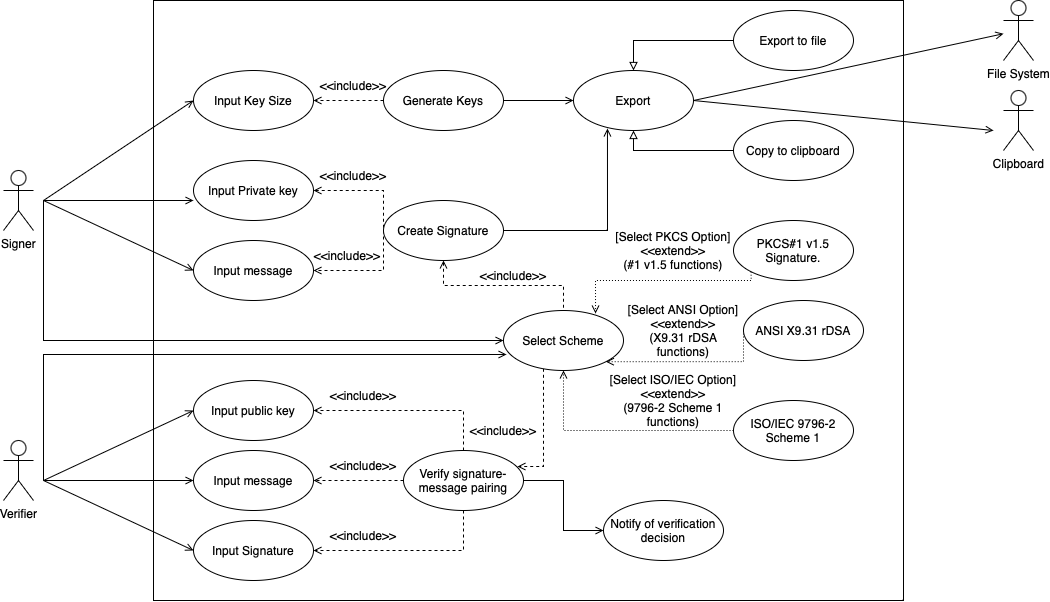
\includegraphics[scale=0.48]{POC_USE-CASE.png}
    \caption{UML Use Case Diagram}
    \label{fig:uc}
\end{figure}

\textbf{Generate Keys Use Case}

\noindent\textbf{Flow of Events:}
\begin{enumerate}
    \item User selects "Generate Key" from the main menu options panel.
    \item User is presented with an input box labeled "Input Key Size".
    \item User inputs desired key size into the box.
    \item System processes the request and generates the public-private key pair.
    \item System displays a notification informing the user that the key generation process was successful.
    \item User is presented with options "Export to file" and "Copy to clipboard".
    \item User selects desired option to either save the keys to a file or copy them to clipboard.
\end{enumerate}

\noindent\textbf{Alternative flows:}
\begin{enumerate}
    \item User inputs an invalid key size.
    \begin{enumerate}
        \item System warns user about the invalid input and prompts them to enter a valid key size again.
        \item System encounters an error during key generation.
        \item System displays an error message and prompts the user to try again.
    \end{enumerate}
\end{enumerate}

\textbf{Create Signature Use Case}

\noindent\textbf{Flow of Events:}
\begin{enumerate}
    \item User selects "Sign message" from the main menu options panel.
    \item User is presented with text boxes labeled "Input Private Key" and "Input Message".
    \item User inputs their private key and the message they wish to sign.
    \item User selects the desired signature scheme from options like "PKCS\#1 v1.5 Signature", "ANSI X9.31 rDSA", etc.
    \item System processes the input and computes the digital signature.
    \item System displays a notification informing the signer that the signing process was successful.
    \item User is presented with options "Export to file" and "Copy to clipboard".
    \item User selects desired option to either save the keys to a file or copy them to clipboard.
\end{enumerate}

\noindent\textbf{Alternative flows:}
\begin{enumerate}
    \item User inputs an invalid or mismatched private key.
    \begin{enumerate}
        \item System warns user about the invalid input and prompts them to enter a valid key.
        \item System encounters an error during signature creation.
        \item System displays an error message and suggests possible solutions or prompts the user to try again.
    \end{enumerate}
\end{enumerate}

\textbf{Verify Signature Use Case}

\noindent\textbf{Flow of Events:}
\begin{enumerate}
    \item User selects "Verify Signature" from the main menu options panel.
    \item User is presented with options to input the message, its corresponding signature, and the public key.
    \item User provides all required inputs.
    \item System processes the information and verifies the authenticity of the signature.
    \item System displays a notification with the result, either confirming the authenticity or notifying of a mismatch.
\end{enumerate}

\noindent\textbf{Alternative flows:}
\begin{enumerate}
    \item User inputs mismatched or incorrect information.
    \begin{enumerate}
        \item System warns user about the incorrect input and suggests rechecking the inputs.
        \item System encounters an error during verification.
        \item System displays an error message and suggests possible solutions or prompts the user to try again.
    \end{enumerate}
\end{enumerate}




%%%% ADD YOUR BIBLIOGRAPHY HERE
\newpage

\addcontentsline{toc}{chapter}{Bibliography}
\printbibliography
\label{endpage}
\end{document}

\end{article}
